\subsection{Analisis \textit{Cost-Sensitive Classification} pada KNN}
\label{subsec:knn-bonus}

Bonus \textit{cost-sensitive classification} pada spesifikasi menetapkan bahwa \textit{false positive} (FP) dua kali lebih mahal dibandingkan \textit{false negative} (FN). Dalam kasus reservasi, FP berarti model memprediksi pembatalan padahal tamu tetap datang, sehingga keputusan menjual ulang kamar dapat menimbulkan \textit{overbooking}. Konsekuensinya, penanganan klasifikasi perlu lebih berhati-hati dalam memberikan label batal. Asumsi biaya yang sama juga dibahas pada tingkat kelompok di Subbab~\ref{sec:cost-sensitive}.

\subsubsection{Perubahan Aturan Keputusan}
Dengan biaya prediksi benar nol, $C_{FP}=2$, dan $C_{FN}=1$, total biaya kesalahan didefinisikan sebagai
\begin{equation}
 C_{\mathrm{total}} = 2FP + FN.
 \label{eq:knn-cost}
\end{equation}
Jika $p$ merupakan estimasi peluang kelas batal, biaya harapan ketika memilih kelas batal adalah $2(1-p)$, sedangkan ketika memilih kelas tidak batal adalah $p$. Aturan yang meminimalkan biaya harapan memilih batal jika
\begin{equation}
 2(1-p)\le p \quad\Longleftrightarrow\quad p\ge\frac{2}{3}.
 \label{eq:knn-threshold}
\end{equation}
Pada KNN, nilai $p$ diestimasi dari proporsi suara tetangga melalui \texttt{predict\_proba}. Untuk $k=7$, aturan mayoritas biasa memerlukan sedikitnya empat tetangga berlabel batal. Ambang $2/3$ mengubah syarat tersebut menjadi \textbf{minimal lima tetangga}. Proporsi suara KNN belum dikalibrasi sebagai probabilitas, sehingga rumus ini dipakai sebagai kebijakan berbasis asumsi biaya yang kemudian diperiksa secara empiris, bukan sebagai jaminan optimum global \cite{elkan2001cost}.

\subsubsection{Hasil dan Analisis}
Simulasi dilakukan pada \textit{holdout} berukuran 5.462 menggunakan konfigurasi 16 fitur, Manhattan, dan $k=7$ yang sama dengan model utama. KNN di-\textit{fit} hanya pada development. Aturan baru diterapkan pada proporsi suara kelas batal tanpa mengubah data latih, hasil \textit{feature selection}, maupun berkas submisi.

\begin{table}[H]
 \centering
 \caption{Perbandingan keputusan KNN standar dan \textit{cost-sensitive} pada \textit{holdout}}
 \label{tab:knn-cost}
 \begin{tabular}{l r r r c}
  \toprule
  \textbf{Aturan keputusan} & \textbf{FP} & \textbf{FN} & \textbf{Total biaya} & \textbf{Macro F1} \\
  \midrule
  Mayoritas standar, minimal 4/7 & 321 & 485 & 1.127 & 0,82830 \\
  \textit{Cost-sensitive}, minimal 5/7 & 177 & 673 & \textbf{1.027} & 0,80791 \\
  \bottomrule
 \end{tabular}
\end{table}

\begin{figure}[H]
 \centering
 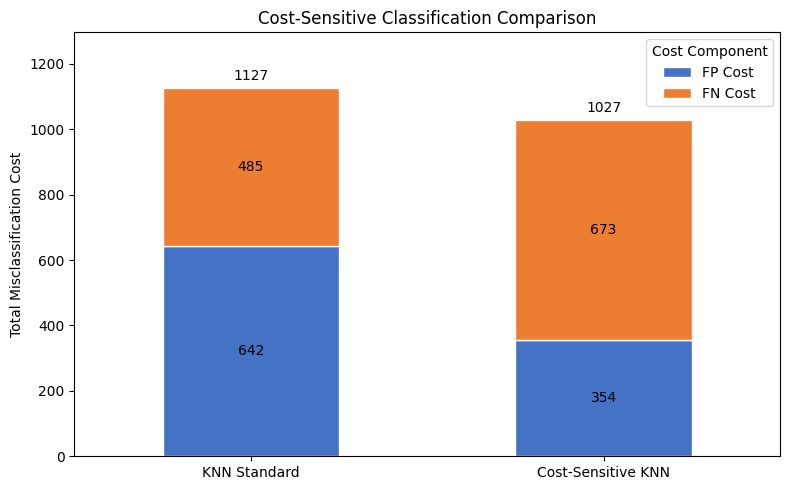
\includegraphics[width=0.72\textwidth]{knn/knn_cost_sensitive.png}
 \caption{Komponen biaya FP dan FN pada aturan mayoritas standar dan \textit{cost-sensitive}}
 \label{fig:knn-cost}
\end{figure}

Perubahan ambang mengurangi FP sebanyak 144 tetapi menambah FN sebanyak 188. Karena satu FP bernilai dua unit biaya, pengurangan FP menghemat 288 unit, sedangkan tambahan FN menambah 188 unit. Biaya bersih turun \textbf{100 unit}, dari 1.127 menjadi 1.027 atau \textbf{8,87\%}. Pada saat yang sama, Macro F1 turun dari 0,82830 menjadi 0,80791. Hasil tersebut menunjukkan bahwa aturan yang lebih sesuai dengan biaya bisnis tidak harus memaksimalkan Macro F1.

Analisis ini merupakan evaluasi tambahan, bukan pelatihan model baru dan bukan submisi Kaggle baru. \texttt{output/knn/submission.csv} tetap memakai keputusan mayoritas standar karena metrik kompetisi adalah Macro F1. Evaluasi dilakukan pada \textit{holdout} yang tidak dipakai memilih ambang $2/3$, sehingga perbandingan memberikan bukti langsung tentang dampak aturan biaya pada konfigurasi KNN yang sudah dipilih.